\documentclass[../1.tex]{subfiles}
\begin{document}

    In this section we shall define structures called simplicial complexes and discuss some of their properties. In order to define these structures
    we need the definitions of convex hull and affine independence in $\R^n$. For a deeper insight into simplicial complexes we refer the reader to 
    \cite{singerthorpe,rotman}.    

    \begin{defn}
        Let $A \subset \R^n$, we define $A$ to be \ii{convex} if
        \[ x,y \in A \then tx + (1+t)y \in A \]
        for all $t \in [0,1]$.
    \end{defn}

    \begin{defn}
        Let $\sigma := \{x_i\}_{i \in I}$ be a finite subset of $\R^n$, we define $\sigma$ to be \ii{affinely independent} if 
        $\{ x_0 - x_i\}_{i \in I - \{0\}}$ is linearly independent.
    \end{defn}

    For the definition of affine independence of $\sigma = \{x_i\}_{i \in I} \subset \R^n$ to be well stated we need it to be independent of the choice of $x_0$.
    In fact had we chosen $x_j$ with $j \in I$, we would have that if $\{ x_j - x_i\}_{i \in I-\{j\}}$ is linearly independent also $\{ x_0 - x_i\}_{i \in I-\{0\}}$ is.
    To prove this let $f : span(\{ x_j - x_i\}) \to span(\{x_0 - x_i\})$ be the identity mapping $(x_j - x_i) \mapsto (x_0 - x_i) - (x_0 - x_j)$, mapping
    the vector $e_i$ in the base $\{ x_j - x_i\}$ to the vector $e_i - e_j$ in the "base" $\{x_0 - x_i\}$. This mapping is represented by the square matrix 
    \[
        F :=
        \begin{pmatrix}
            I & \cdots & O \\
            -1 & \cdots & -1\\
            O & \cdots & I
        \end{pmatrix},
    \]
    where the j-th raw is $(-1,...,-1)$.
    Adding all the raws to the j-th we obtain the diagonal matrix $diag(1,...,1,-1,1,...,1)$, therefore $detF = -1$.
    From the non-zero determinant we can conclude that $f$ is an isomorphism, which makes our definition well stated.

    \begin{defn}
        Let $\sigma := \{x_i\}_{i \in I}$ be a finite subset of $\R^n$, we define the \ii{covex set generated by $\sigma$} to be 
        the smallest convex set containing $X$ according to the inclusion relation.
    \end{defn}

    Since the intersection of convex sets is convex, the convex set generated by $\sigma$ can be equivalently defined as the intersection 
    of all convex sets containing $\sigma$.

    \begin{thm}
        Let $\sigma := \{x_i\}_{i \in I}$ be a finite subset of $\R^n$, if $X$ is affinely independent then the convex set generated by $X$ is 
        \[ [\sigma] := \{ \sum_{i \in I} \lambda_i x_i : \lambda_i \geq 0, \sum_{i \in I} \lambda_i = 1\}. \]
        Furthermore for any point $x \in [\sigma]$ we have that
        \[ x = \sum_{i \in I} \lambda_i x_i = \sum_{i \in I} \mu_i x_i \then \lambda_i = \mu_i \forall i \in I, \] 
        where $\lambda_i,\mu_i \geq 0$ and $\sum_{i \in I} \lambda_i = \sum_{i \in I} \mu_i =1$.
        \label{thm:1}
    \end{thm}

    \begin{proof}
        Let $C := \{ \bigcap_\alpha C_\alpha : \sigma \in C_\alpha, C_\alpha$ convex$\}$, we want to show that:
        \begin{enumerate}[(i)]
            \item $C \subset [\sigma]$\\
            This is true if $[\sigma]$ is convex and contains $\sigma$.
            The proof that it contains $\sigma$ is trivial. In fact for every vertex $x_j = \sum_{i \in I} \delta_{ij} x_i$,
            and $\sum_{i \in I}\delta_{ij} = 1$.\\
            To prove that it is convex we chose two points $a = \sum_{i \in I} a_i x_i, b = \sum_{i \in I} b_i x_i$ where $a_i,b_i \geq 0 \forall i \in I$
            and $\sum_{i \in I} a_i = \sum_{i \in I} b_i = 1$. For $t \in [0,1]$
            \[ ta+(1-t)b = t\sum_{i \in I} a_i x_i + (1-t) \sum_{i \in I} b_i x_i = \sum_{i \in I} (ta_i + (1-t)b_i)x_i.\]
            It follows that $ta_i + (1-t)b_i \geq 0$ and $\sum_{i \in I} (ta_i + (1-t)b_i) = t\sum_{i \in I}a_i + (1-t)\sum_{i \in I}b_i = 1$ for all $i \in I$,
            therefore (i) is proven.

            \item $[\sigma] \subset C$
            \item $\sum_{i \in I} \lambda_i x_i = \sum_{i \in I} \mu_i x_i \then \lambda_i = \mu_i \forall i \in I$
        \end{enumerate}
    \end{proof}

    A proof of theorem \ref{thm:1} can be found in \cite{singerthorpe}.
    The set $[\sigma]$ is often called \ii{covex hull} of $\sigma$.
    
    \begin{exa}
        Let ${A,B,C,D} \subset \R^n$ representing the four vertxes of a square and let $A,D$ be opposite vertxes, one can easily see that 
        \[ D = A + (B-A) + (C-A) = (-1)A + (1)B + (1)C + (0)D = (0)A + (0)B + (0)C + (1)D \, ,\]
        therefore $A,B,C,D$ are not affinely independent.
        In fact the $4$ vertexes of a square are coplanar, i.e. they belong to the same $2$ dimensional affine space.
    \end{exa}

    % image

    \begin{defn}
        We define a \ii{p-simplex} $[\sigma]$ to be the convex hull of an affinely independent set $\sigma := \{x_i\}_{i \in I} \subset \R^n$,
        where $p = |I|-1$ is called dimension of the p-simplex. 
    \end{defn}

    Theorem \ref{thm:1} gives us the possibility to represent a point in a simplex $[\sigma]$ via a finite set of real parameters defined in the range $[0,1]$
    and satisfying the normalisation condition $\sum_{i \in I } \lambda_i = 1$. Such parameters are called \ii{baricentric coordinates} of $[\sigma]$.\\
    \hfill \\
    The points in $\sigma$ are called \ii{vertexes} of the simplex $[\sigma]$, accordingly we define the vertex set of a simplex $[\sigma]$ to be 
    $Vert([\sigma]) = \sigma$.
    
    \begin{defn}
        Let $[\sigma]$ be a p-simplex and $p,t \in \N$, we say that another t-simplex $[\tau]$ is a \ii{face} of $[\sigma]$ or equivalently 
        that $[\sigma]$ is a \ii{coface} of $[\tau]$, and we write $[\tau] \leq [\sigma$], if $\tau \subset \sigma$, where $t \leq p$.
    \end{defn}

    Now we are ready for our main definitions.
    
    \begin{defn}
        We define a \ii{simplicial complex} $\mc{G}$ to be a collection of simplexes such that
        \begin{enumerate}[(i)]
            \item if any simplex $ [\tau] \leq [\sigma], [\sigma] \in \mc{G}$ then $ [\tau] \in \mc{G}$,
            \item if $ [\sigma], [\tau] \in \mc{G}$ then $[\sigma] \cap [\tau] \in \mc{G}$.
        \end{enumerate}
    \end{defn}

    
    \begin{figure}[h]
        \centering
        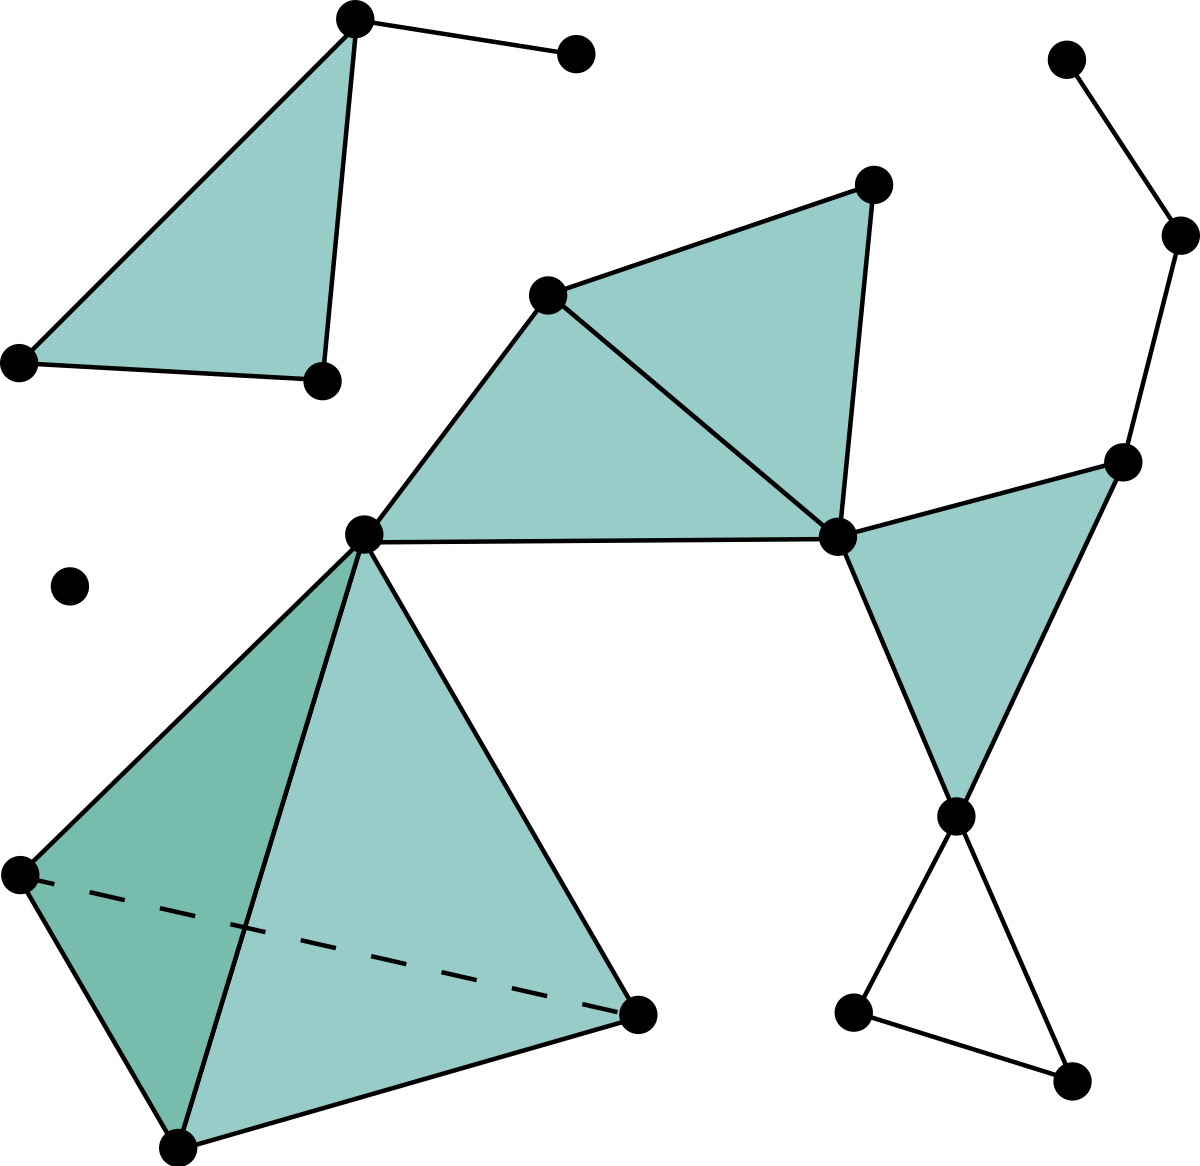
\includegraphics[width=4cm, height=4cm]{sections/1/complex}
        \caption{Example of simplicial complex.}
        \label{fig:1}
    \end{figure} 

    \begin{figure}[h]
        \centering
        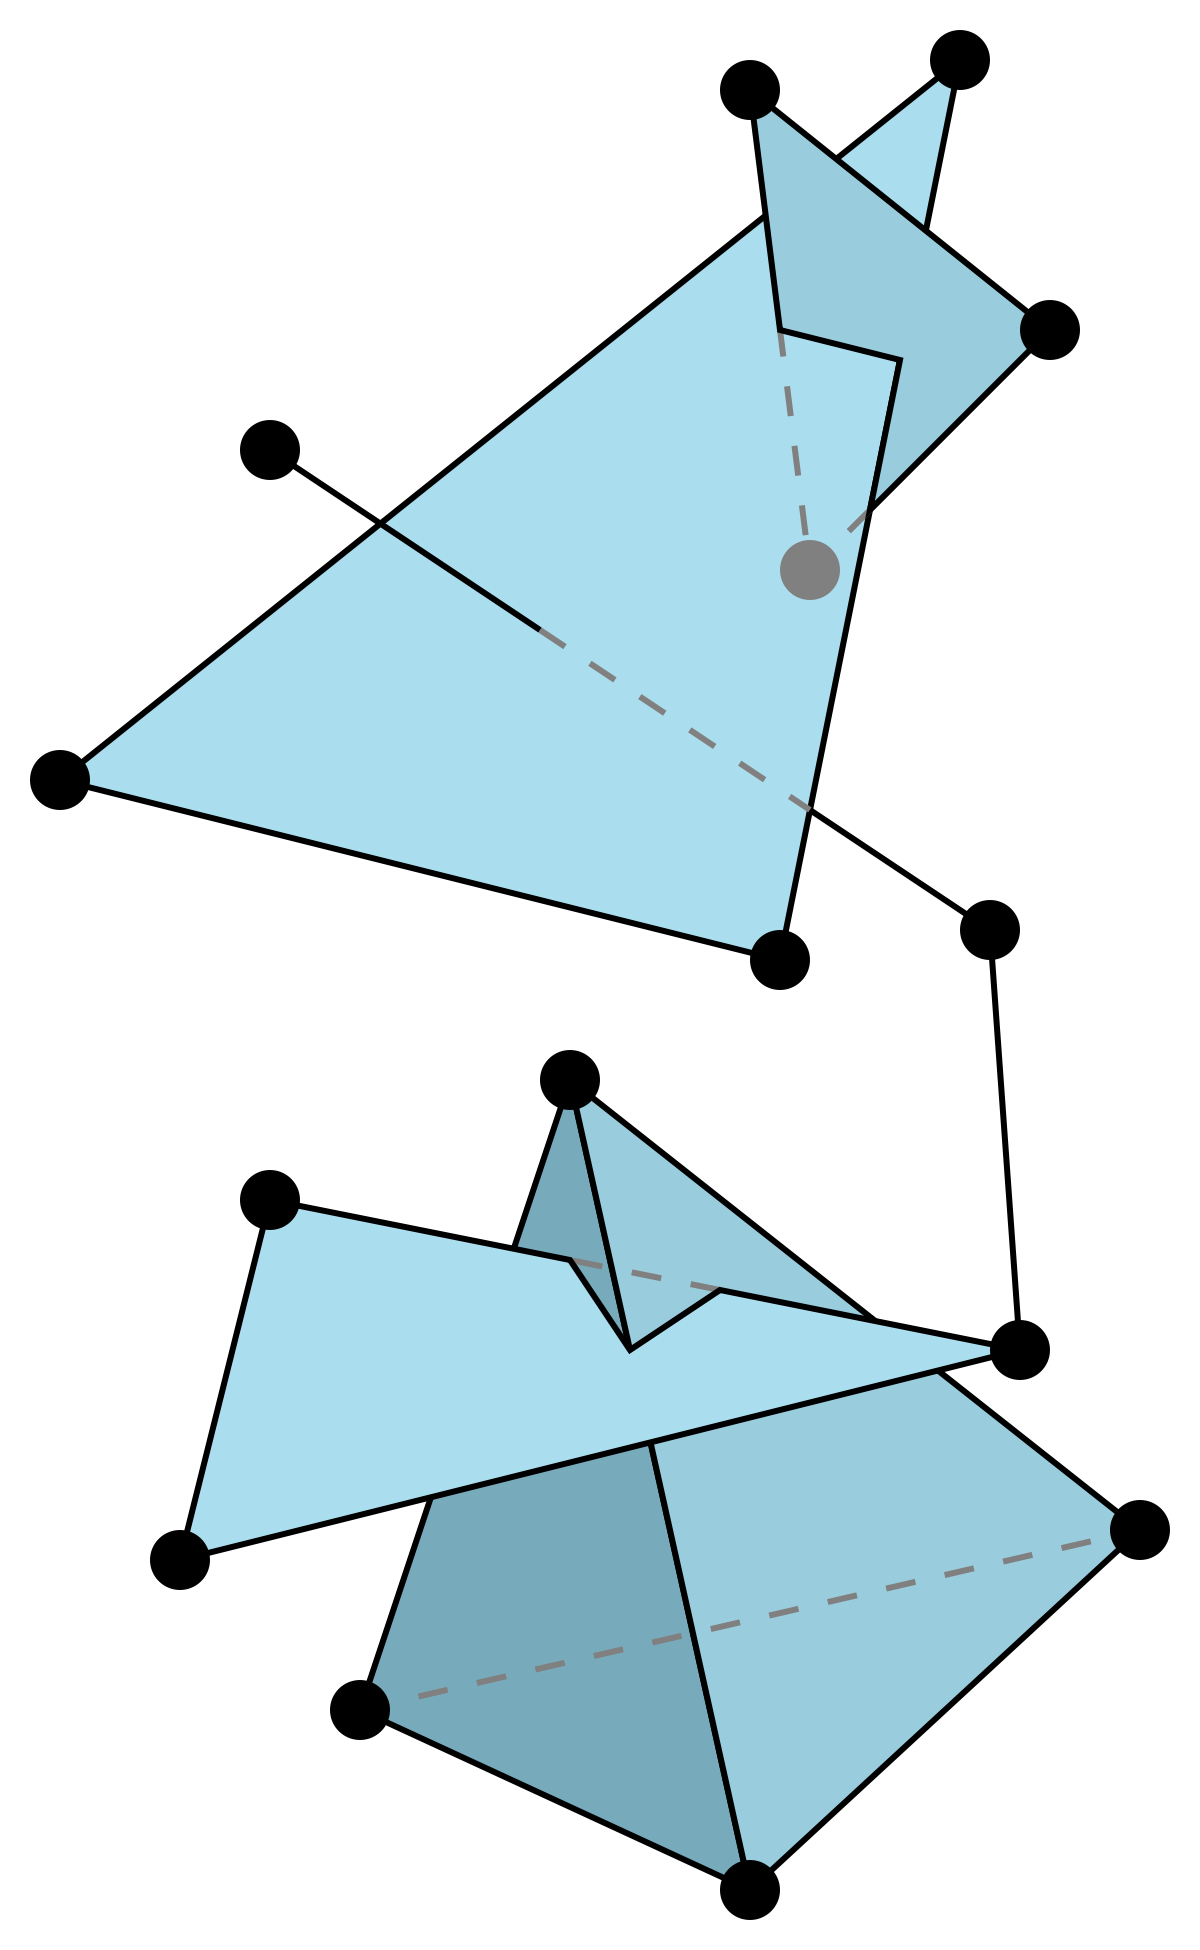
\includegraphics[width=3cm, height=5cm]{sections/1/noncomplex}
        \caption{Set of simplexes which is not a simplicial complex.}
        \label{fig:2}
    \end{figure}

    We can see in Fig. \ref{fig:2} that the intersection property of simplicial complexes is not satisfied.\\
    \hfill \\
    % Simplicial complexes are the objects of our category, we now look for appropriate morphisms.

    % \begin{defn}
    %     Let $\mc{G},\mc{H}$ be simplicial complexes, then a \ii{simplicial map} $\phi : \mc{G} \to \mc{H}$ is a function 
    %     such that whenever $[ x_i ]_{i \in I} \in \mc{G}$, then $\phi([ x_i ]_{i \in I}) = [ \phi(v_i) ]_{i \in I} \in \mc{H}$,
    %     where $\phi(x_i) \in Vert(\mc{H}) \, \forall i \in I$.
    % \end{defn}

    % \begin{thm}
    %     Simplicial complexes and simplicial maps are a category $\bb{G}$, whose equivalences are called isomorphisms..
    % \end{thm}

    % \begin{defn}
    %     Let $\mc{G}$ be a simplicial complex, we define its \ii{underlying space} $|\mc{G}| = \bigcup_{\sigma \in \mc{G}} \sigma$, provided with
    %     the standard topology inherited from $\R^n$.
    % \end{defn}

    % Since the union of compact sets is compact the underlying space of a simplicial complex in $\R^n$ is a compact topological subspace of $\R^n$.

    % \begin{defn}
    %     A topological space $X$ is called \ii{polyhedron} if there exists a simplicial complex $\mc{G}$ and a homeomorphism
    %     $h : |\mc{G}| \to X$. The ordered pair $(\mc{G}, h)$ is called a \ii{triangulation} of $X$.
    % \end{defn}

    % One understands that in order to have a homeomorphism between the compact underlying space of a simplcial complex and another topological
    % space, this other space has to be compact.

    % \begin{lem}
    %     Let a topological space $X$ be a finite union of closed subsets $X = \bigcup_{i \in I} X_i$. If, for some space Y, there are continuous
    %     maps $f_i : X_i \to Y$ that agree on overlaps $f_i |_{X_i \cap X_j} = f_j |_{X_i \cap X_j}$, there there exist a unique continuous
    %     function $f : X \to Y$ such that $f |_{X_i} = f_i \, \forall i \in I$.
    % \end{lem}

    % \begin{defn}
    %     Let $\phi : \mc{G} \to \mc{H}$ be a simplicial map, let then $\sigma \in \mc{G}$ we define $f_\sigma : \sigma \to |\mc{H}|$ to be 
    %     $\sum_{v \in Vert(\sigma)} \lambda_v v \mapsto \sum_{v \in Vert(\sigma)} \lambda_v \phi(v)$. The continuity of this functions in $\sigma$ and the
    %     intersection property of the definition of simplicial complex allow us to use the previous lemma to uniquely define a function $|\phi| : |\mc{G}| \to |\mc{H}|$
    %     which we shall name \ii{piecewise linear map}.
    % \end{defn}

    % The unique association of simplicial complexes and their underlying spaces and of simlicial maps and piecewise linear maps leads to the definition
    % of a functor from the category of simplicial complexes and maps to the category of topological spaces and continuous functions.

    % \begin{thm}
    %     $|\;| : \bb{G} \to \bb{Top}$ is a functor.
    % \end{thm}

    % Notice that there is no obvious functor from $\bb{Top}$ to $\bb{G}$, therefore the implications reguarding equivalences are strictly directed.\\

    Although this approach provides simplicial complexes with the topology inherited from the metric space, it hides the power of simplicial complexes 
    to describe those networks and interactions which would happily exist without that topology. To make this distinction clear enough we will treat
    simplicial complexes as a realization of more abstract objects called abstract simplicial complexes. The discussion of abstract simplicial complexes
    can be found in \cite{rotman}.
    
    \begin{defn}
        Let $\mc{V}$ be a finite set we define an \ii{abstract simplicial complex} $\mc{A}$ to be 
        \[\mc{A}:=\{ \sigma  \subset \mc{V} : \tau \subset \sigma \then \tau \in \mc{A} \}\] 
        where $\sigma$ are called \ii{abstract simplexes} of $\mc{A}$.
    \end{defn}
    
    One calls $\mc{V}$ the \ii{vertex set} of $\mc{A}$ and denotes it by $Vert(\mc{A})$; since the vertex
    set is finite we expect every abstract simplex to be also finite, therefore we might use the notation $\sigma = \{ v_i \}_{i \in I_\sigma}$,
    which so far we consider invariant under arbitrary permutations of the finite index set $I_\sigma$.

    \begin{defn}
        Let $\mc{A}$ be an abstract simplicial complex we define its \ii{dimension} to be
        \[ dim \mc{A} := max_{\sigma \in \mc{A}}(|\sigma|-1), \]
        where by $|\sigma|$ we denote the cardinality of $\sigma$.
    \end{defn}

    One calls an abstract simplex of dimension $p$ an \ii{abstract p-simplex}, according to our
    definition the empy set is a $(-1)$-simplex. A \ii{graph} is a one dimensional abstract simplicial complex.

    % \begin{defn}
    %     Let $\mc{A},\mc{B}$ be abstract simplicial complexes, then a \ii{simplicial map} $\phi : \mc{A} \to \mc{B}$ is a function 
    %     such that whenever $\sigma = \{v_i\}_{i \in I_\sigma} \in \mc{A}$, then $\phi(\{v_i\}_{i \in I_\sigma}) = \{\phi(v_i)\}_{i \in I_\sigma} \in \mc{B}$,
    %     where $\phi(v_i) \in Vert(\mc{B}) \, \forall i \in I_\sigma$.
    % \end{defn}

    % Although the vertex to vertex mapping is a quite selective condition on the function we did not prevent it from cramming
    % abstract simplexes into lower dimensional ones.

    % \begin{thm}
    %     Abstract simplicial complexes and simplicial maps are a category $\bb{A}$, whose equivalences are called isomorphisms.
    % \end{thm}

    % One can show that under some dimensional conditions one can define a functor from the category of abstract simplicial complexes
    % to the category of simplicial complexes.

    % \begin{defn}
    %     Let $\mc{G}$ be a simplicial complex,  we call the abstract simplicial complex 
    %     \[ \mc{A} := \{ \{x_i\}_{i \in I} \subset Vert(\mc{G}) : [x_i]_{i \in I} \in \mc{G} \} \]
    %     a vertex scheme for $\mc{G}$ or equivalently we might say that $\mc{G}$ is a \ii{geometric realization} of $\mc{A}$.
    % \end{defn}

    % \begin{thm}
    %     Let $\mc{A}$ be a d-dimensional abstract simplicial complex, it admits a geometric realization in $\R^{2d+1}$.
    % \end{thm}
    % Kuratowski theorem proves the prevuois statement to be also sharp.\\
    % \hfill \\
    % One could also show that that geometric realizations of isomorphic abstract simplicial complexes are themselves isomorphic.
\end{document}
